\documentclass[12pt]{report}
\usepackage{amsmath}
\usepackage{amsfonts}
\usepackage{amssymb}
\usepackage{textcomp}
\usepackage{graphicx}
\usepackage{float}
\usepackage{hyperref}
\usepackage[a4paper, margin = 1in]{geometry}

\usepackage[draft]{todonotes}


%Commands used in text, edit here and the document will populate with correct value.
\newcommand{\projectName}{CEPAD }
\newcommand{\payLoadMass}{3.352Kgs }

%*******************************TITLE PAGE*******************************%

\title{Development of a Close Quarter Collision Protected Aerial Drone}
\author{Angus Steele} 

\begin{document}
	\section{Altitude Controller}
	This section discusses the implementation of the altitude controller. The overall altitude controller is structured as a set of cascaded control loops, with the most inner loop controlling the aircraft's acceleration and the most outer loop controlling the desired altitude in the earth frame. In order to control the altitude of a craft, an analysis of the system's heave dynamics must first be performed. Once a mathematical model has been created, an inner PI heave controller is applied to follow a desired vertical acceleration reference. The climb rate P controller is responsible for generating these acceleration references and is fed a desired linear vertical velocity reference by the altitude hold P controller. 
	
	\subsection{Heave Dynamics}
	Using Newton mechanics at near hover conditions for the aircraft, the heave dynamics can be derived and are shown in \eqref{EQ_HeaveNewton}. Where $\dot{W}$ is the current acceleration of the craft in the Z-Axis and $m$ is the vehicles's mass. $Z$ is defined as the current instantaneous force being produced by the rotors.
	
	\begin{equation}
	\label{EQ_HeaveNewton}
	\dot{W} = \dfrac{Z}{m}
	\end{equation}
	
	The state variable of the system is chosen as $Z$ with the output of this plant being $\dot{W}$. Using the transfer function for motor-rotor lag dynamics seen in \eqref{EQ_MotorDelay} and the dynamics seen in \eqref{EQ_HeaveNewton}, the state space equation for the system can be derived and is shown in \eqref{EQ_HeaveStateSpace1} and \eqref{EQ_HeaveStateSpace2}. 
	
	\begin{eqnarray}
	[\dot{Z}] &=& - [\dfrac{1}{\tau}] \ [Z] + [\dfrac{1}{\tau}] [\delta_Z]\label{EQ_HeaveStateSpace1}\\\label{EQ_HeaveStateSpace11}
	[\dot{W}] &=& - [\dfrac{1}{m}] \ [Z]\label{EQ_HeaveStateSpace2}
	\end{eqnarray}
	
	Subsequently the transfer function can be calculated and the result is shown in \eqref{EQ_HeaveTF}. The negative gain of the transfer function must be noted and is caused by the direction of the defined axes, with the rotors producing a negative Z-Axis force.
	
	\begin{equation}
	G(s)_{heave} = \frac{\frac{-1}{m \times \tau}}{s + \frac{1}{\tau}}\label{EQ_HeaveTF}
	\end{equation}
	
	The rotor motor lag produces the pole at $\dfrac{-1}{\tau} = -8$ and indicates the maximum response capabilities and timing constant of the rotor system.
	
	\subsection{Heave Controller}
	The heave controller is responsible for commanding the $\delta_Z$ virtual actuator to achieve a desired Z-Axis acceleration in the body frame. The model derived above can be shown to produce a large steady state error. A PI architecture was initially chosen as shown in Figure \ref{IM_HeaveController}. 
	
	The integrator is used to remove the steady state error, while the most left limiter shown in Figure \ref{IM_HeaveController} was added to stop integrator wind up and is not considered during the linear controller design. The proportional gain is used to move the closed loop poles and achieve the desired bandwidth. The dynamic response of the system can be investigated using the root locus and bode plots shown in Figure \ref{IM_HeaveControlRoot} and \ref{IM_HeaveControlBode}. 
	
	\begin{figure}[H]
		\centering
		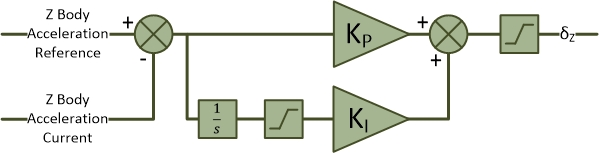
\includegraphics[height = 3.5cm]{../References/Diagrams/HeaveController.jpg}
		\caption{Heave Controller -  Control Diagram}
		\label{IM_HeaveController}
	\end{figure}
	
	Figure \ref{IM_HeaveControlRoot} shows the root locus of the system with the PI controller included. The controller introduces a new pole at the origin. To maintain a first order response, the zero is placed close to the plant pole. This placement will attenuate the open loop, plant pole's response. Finally the gain is varied until the closed loop responses are closely aligned with the naturally occurring open loop pole. The final closed loop poles are a set of complex poles and are located at $-7.55 \pm 3.64 i$. The frequency response can be evaluated using the bode plot in Figure \ref{IM_HeaveControlBode}. 
	
	\begin{figure}[H]
		\centering
		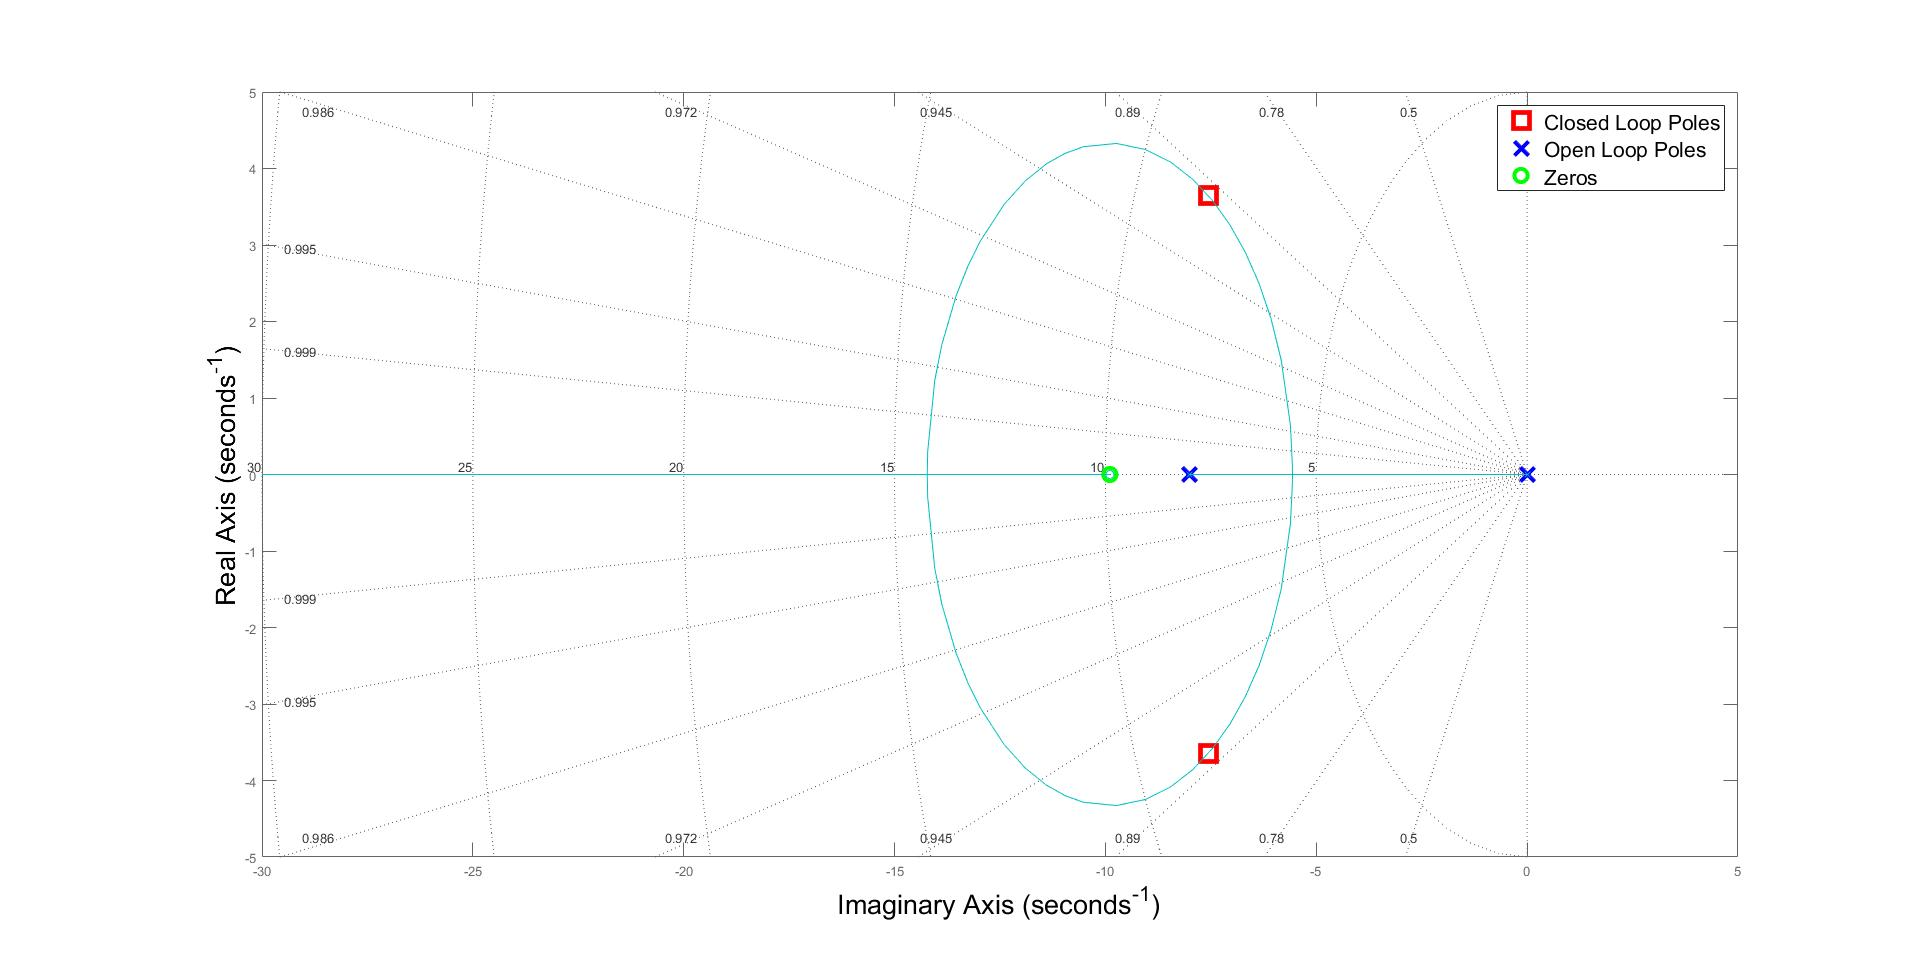
\includegraphics[height = 8cm]{../Design/Matlab/Controllers/heave_root.jpg}
		\caption{Heave Controller -  Root Locus}
		\label{IM_HeaveControlRoot}
	\end{figure}
	
	The final cross over frequency is shown on the bode plot for the heave controller in Figure \ref{IM_HeaveControlBode}. The gain plot shows the controller adjust the crossover frequency to $7.99 Rad/s$ which is close to the limit of the system. The controller also increases the phase of the system and has a final phase margin of $83.96$\textdegree. The resultant control law is shown in \eqref{EQ_HeaveController}.
	
	\begin{equation}
	\label{EQ_HeaveController}
	C(s)_{heave} = \frac{2.9782 (s + 9.985)}{s}
	\end{equation}		
	
	\begin{figure}[H]
		\centering
		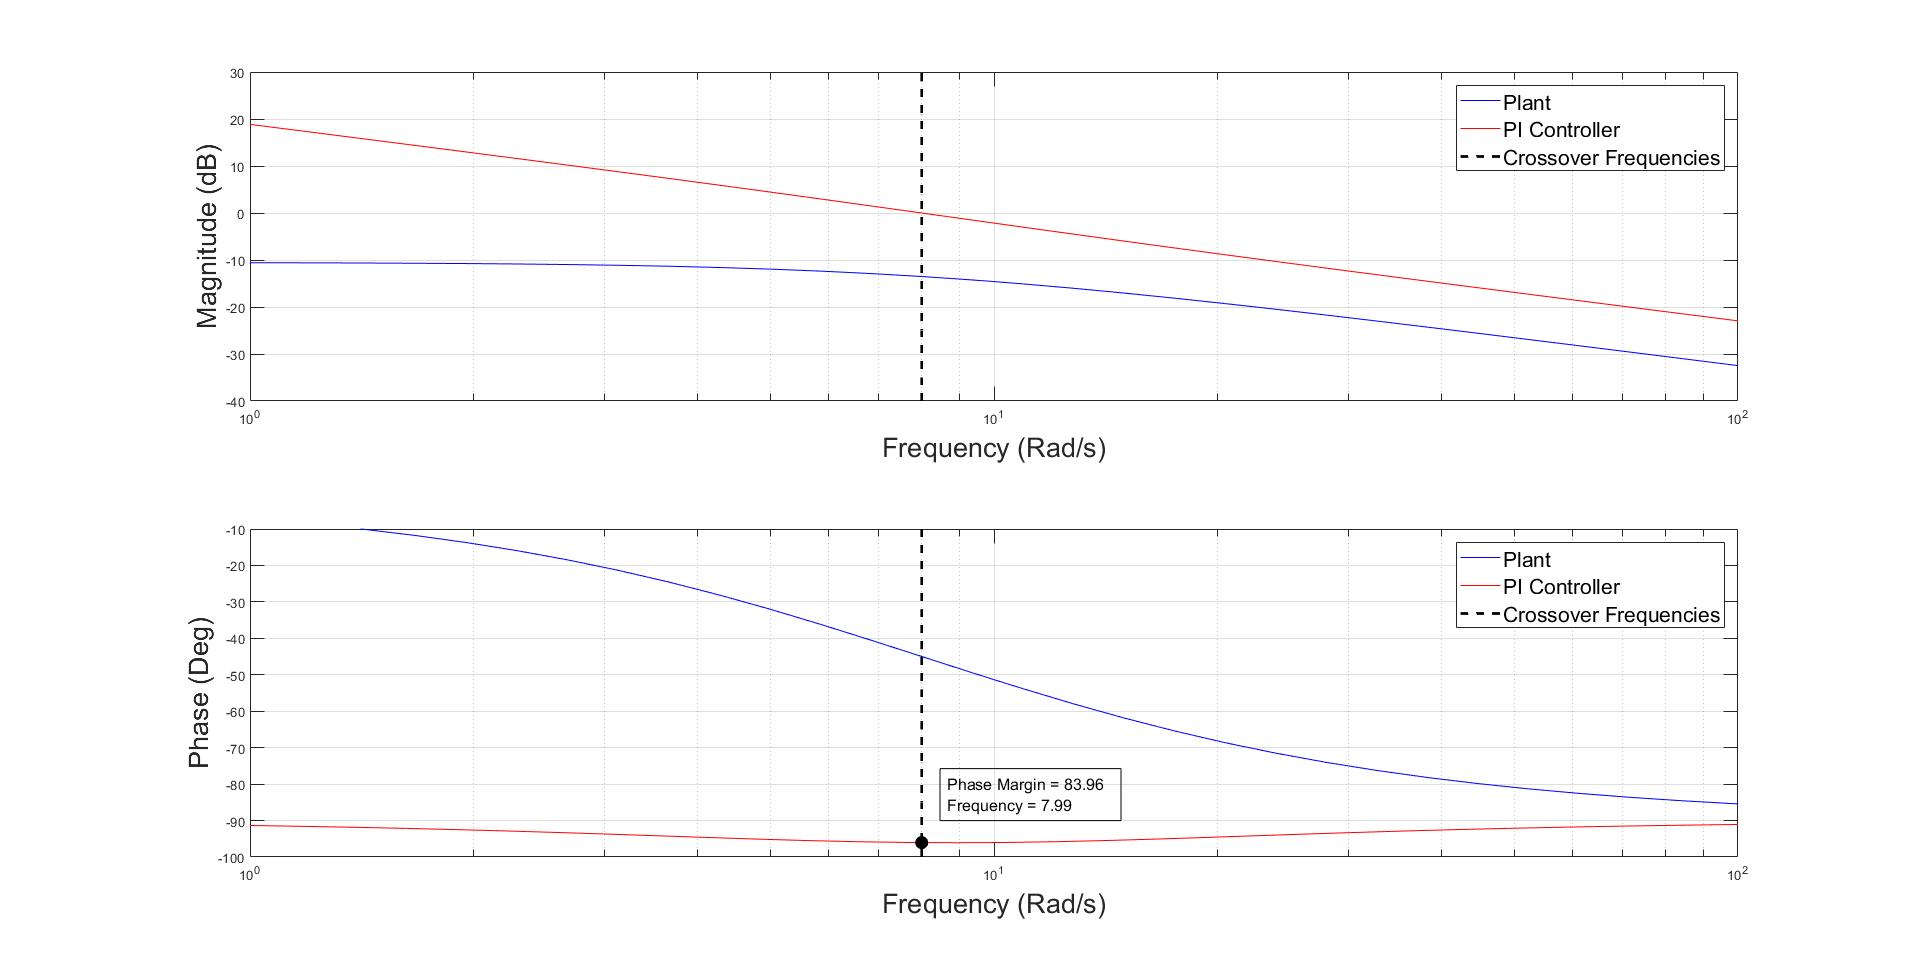
\includegraphics[height = 8cm]{../Design/Matlab/Controllers/heave_bode.jpg}
		\caption{Heave Controller -  Bode Plots}
		\label{IM_HeaveControlBode}
	\end{figure}
	
	An additional non linear element in the form of a limiter is brought into the system to limit the maximum and minimum thrust commands. The maximum limit is used to ensure the heave controller does not saturate the motors. This creates headroom for the angular rate controllers and disturbance rejection. The lower limit is used to ensure the vehicle always descends at a steady pace. The maximum thrust capabilities are displayed in table \ref{tab:ThrustProfiles}, summing these values produces a total maximum thrust of approximately $76N$ for the total rotor system. The final limits chosen are shown in Table \ref{tab:HeaveLimits}.
	
	\begin{table}[!]
		\centering
		\begin{tabular}{l | c | c |}
			Limit Name 				& Min & Max\\
			\hline\hline
			Integrator Wind Up 	   	& -1.5 	& 1.5 \\
			Thrust Command 		    & 10	& 55 \\
		\end{tabular}
		\caption{Heave Controller Limits}
		\label{tab:HeaveLimits}
	\end{table}
	
	
	
	\subsubsection{Heave Controller Discussion}
	Now that the system presents stable dynamic results in the frequency and Laplace domains, using the non-linear simulation, the time domain responses can be discussed in brief. The resultant step response, including the PI controller, is shown in Figure \ref{IM_HeaveStepDist}. To demonstrate the disturbance rejection capabilities of the design, a force of $10N$ is applied to the drone at $2.5s$.
	
	\begin{figure}[H]
		\centering
		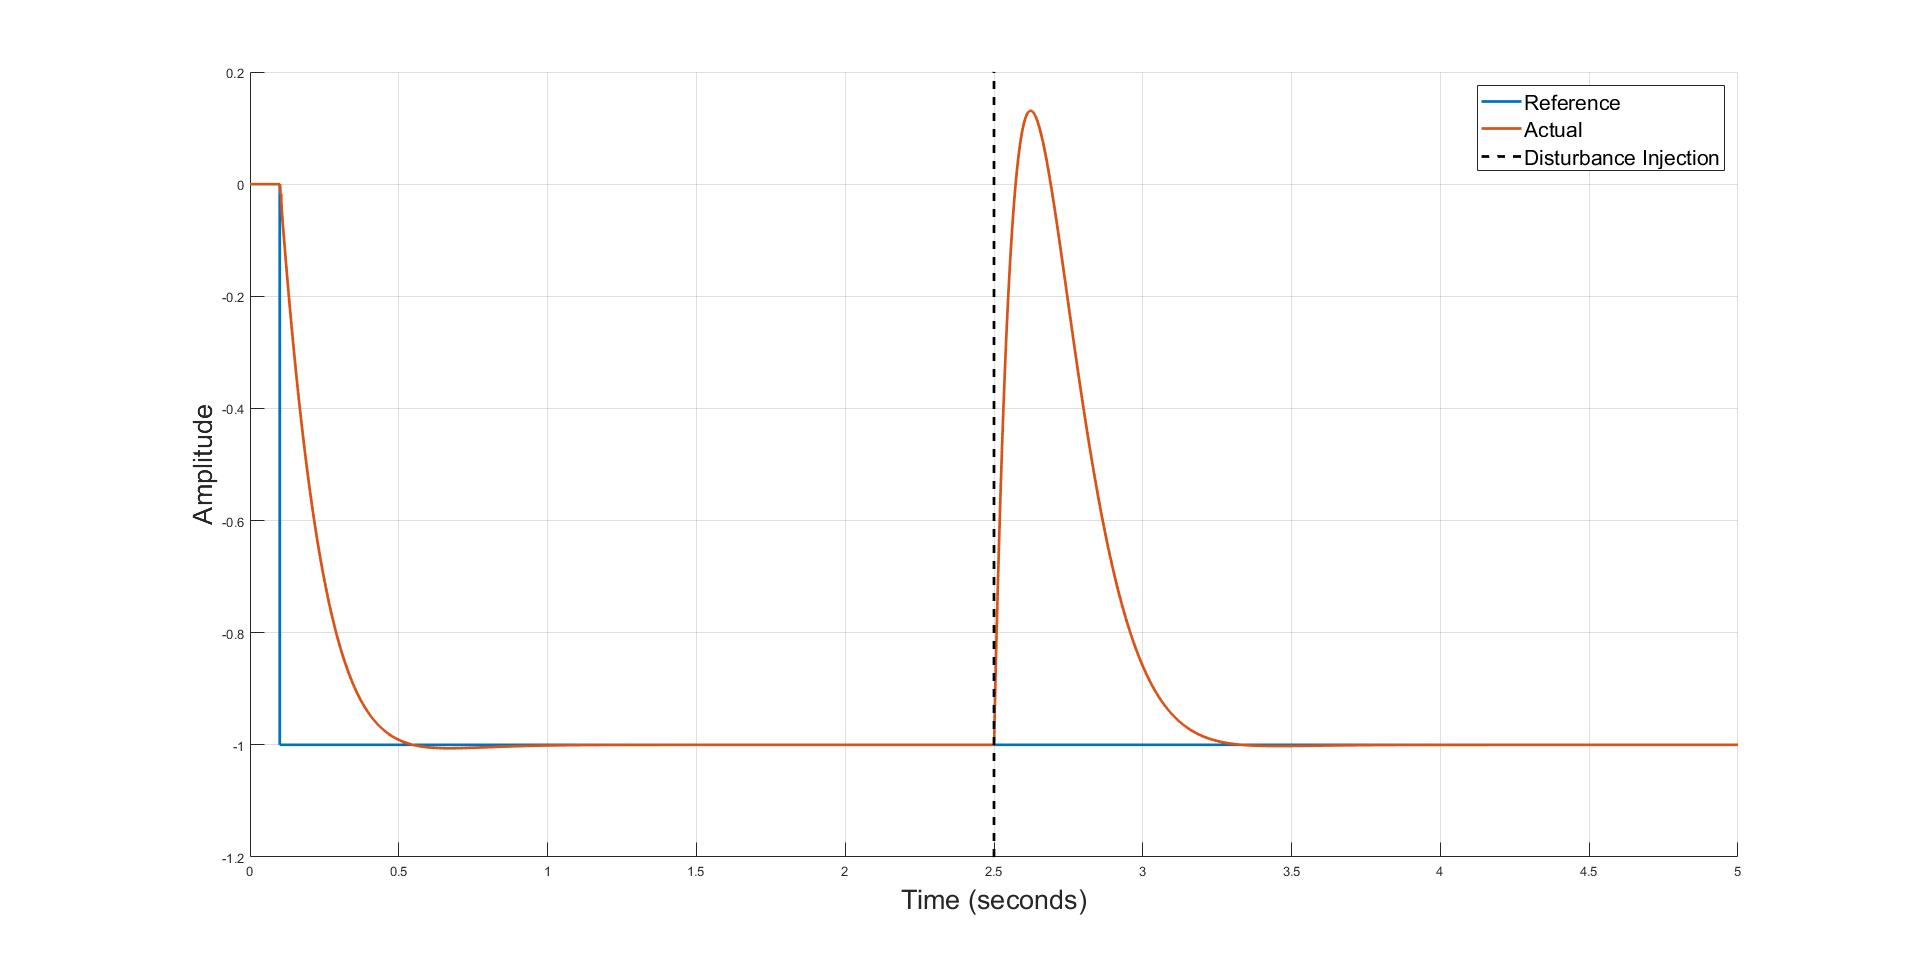
\includegraphics[height = 8cm]{../Design/Matlab/Controllers/heave_step.jpg}
		\caption{Heave Controller -  Step Response}
		\label{IM_HeaveStepDist}
	\end{figure}
	
	The heave controller, as the most inner loop, limits the response for the rest of the altitude control system. The proposed design brings the heave loop response close to the limits of the plant, thus producing a similar (but slower) timing constant to that of the motor-rotor system. The system reaches and settles within 5\% of the reference by $0.313s$, is critically damped and presents negligible overshoot. The system also shows to be capable of tracking an acceleration setpoint with zero steady state error. As shown in Figure \ref{IM_HeaveStepDist} the system can also respond quickly to a large, sudden and constant disturbance.
	
	\subsection{Climb Rate Controller}
	The climb rate controller is responsible for controlling the vertical velocity of the aircraft, in the earth frame. This introduces the need for rotating either the reference or the command into the body frame. The decision can be made by considering the frame in which the sensing information is provided. Most aircraft make use of some form of global positioning system and using differentiation can calculate speed. However, due to the application environment, this aircraft will most likely use a velocity measurement sensor relative to the body frame. The architecture for the climb rate controller is outlined in Figure \ref{IM_ClimbRateControlLoop}. 
	
	The speed of the climb rate controller is limited by the inner heave leave control loop, this becomes a limiting design criterion for the system.
	
	\begin{figure}[H]
		\centering
		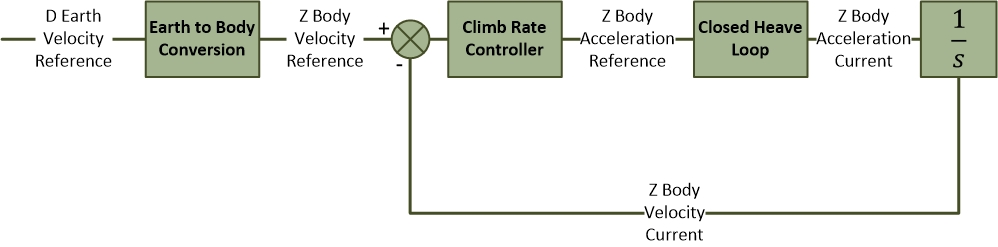
\includegraphics[height = 3.75cm]{../References/Diagrams/ClimbRateLoop.jpg}
		\caption{Climb Rate Controller Closed Loop}
		\label{IM_ClimbRateControlLoop}
	\end{figure}
	
	At near hover conditions the plant can be linearised and the rotation can be excluded. Figure \ref{IM_ClimbRateController} shows the simplified climb rate controller architecture. The computational time required for rotating the references can be considered by ensuring the controller design provides a reasonable phase margin. The open loop poles of the climb rate system are located at the closed loop pole positions of the inner heave system, while the mathematical relationship between acceleration and velocity yields an additional open loop pole at the origin.
	
	\begin{figure}[H]
		\centering
		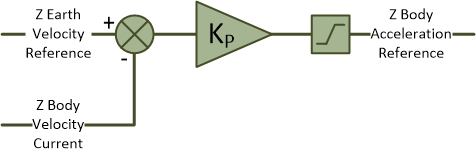
\includegraphics[height = 3.5cm]{../References/Diagrams/ClimbRateController.jpg}
		\caption{Climb Rate Controller}
		\label{IM_ClimbRateController}
	\end{figure}		
	
	The free integrator in the plant ensures the system will track a step response with zero steady state error while the proportional gain is used to speed up the system and achieve the desired bandwidth.
	The dynamic response of the system, including the controller, is evaluated using the root locus and bode plots shown in Figure \ref{IM_ClimbRateRoot} and \ref{IM_ClimbRateBode}.
	
	\begin{figure}[H]
		\centering
		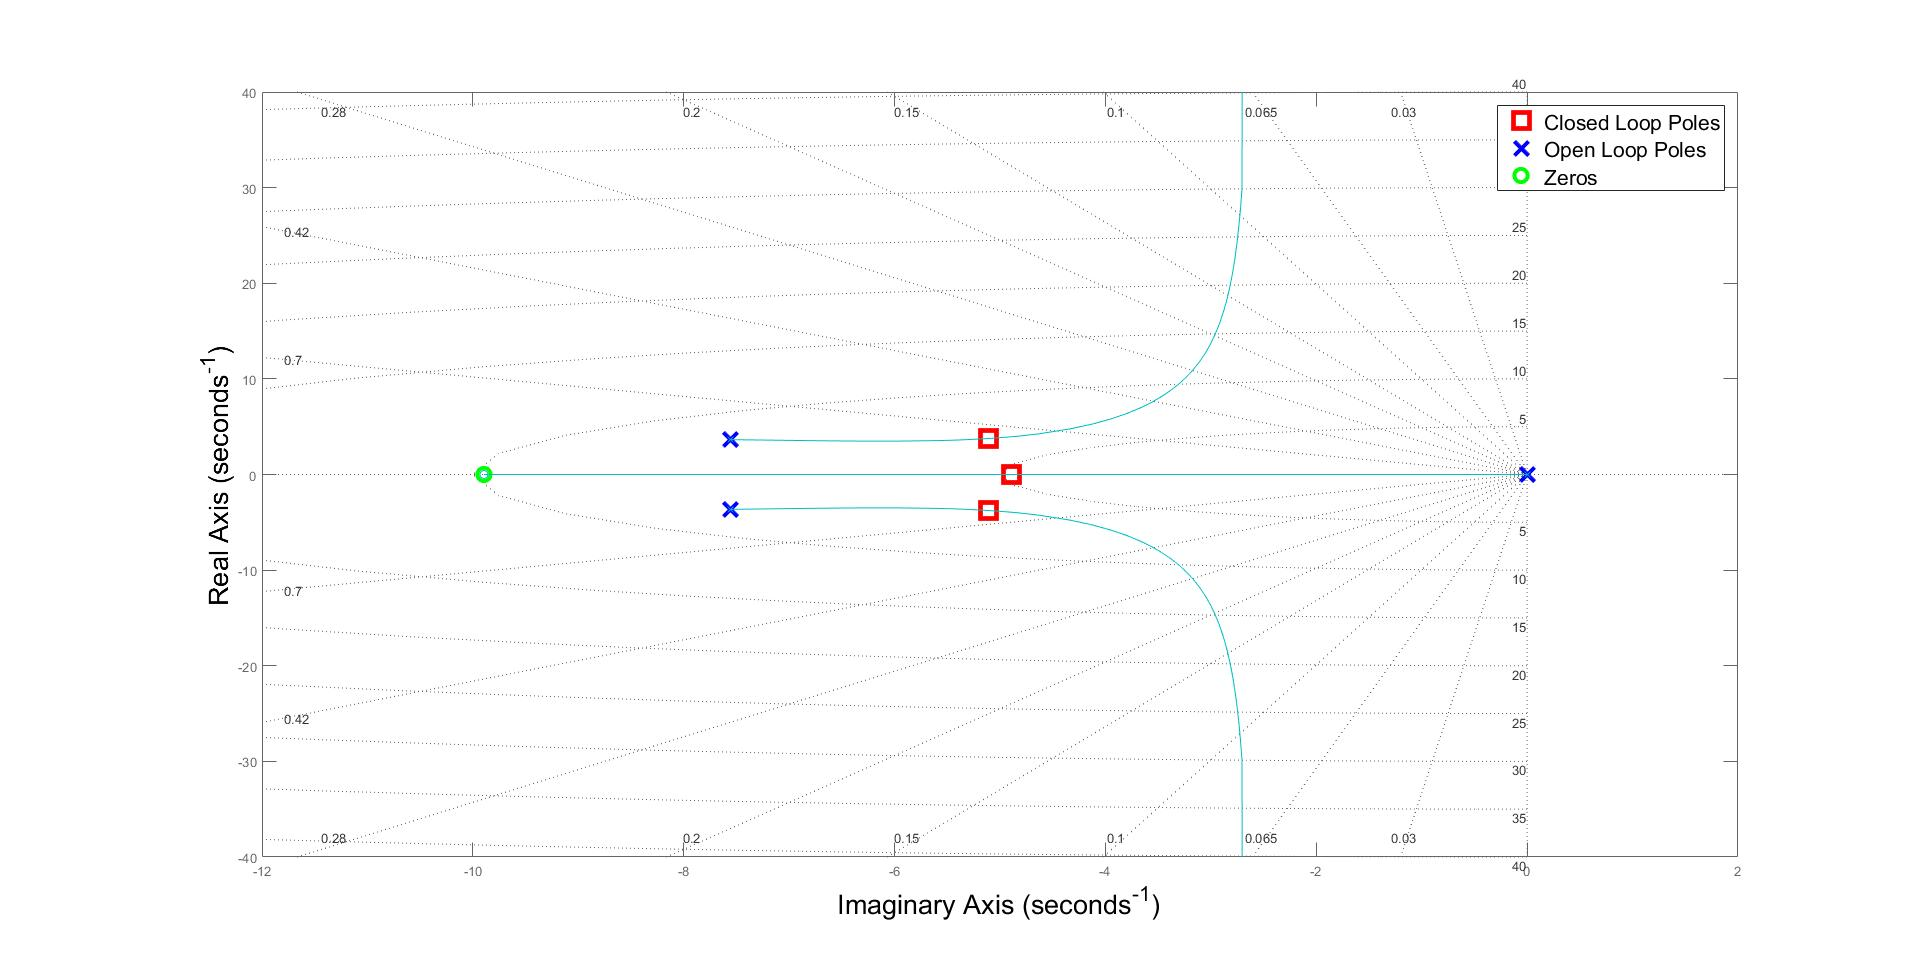
\includegraphics[height = 8cm]{../Design/Matlab/Controllers/climb_rate_root.jpg}
		\caption{Climb Rate Controller -  Root Locus}
		\label{IM_ClimbRateRoot}
	\end{figure}
	
	Figure \ref{IM_ClimbRateRoot} shows the location of the three final closed loop poles. The complex pair is placed at $-5.11 \pm 3.76i$ and the integrator pole is located at $-4.89$ and is on the imaginary axis.
	
	\begin{figure}[H]
		\centering
		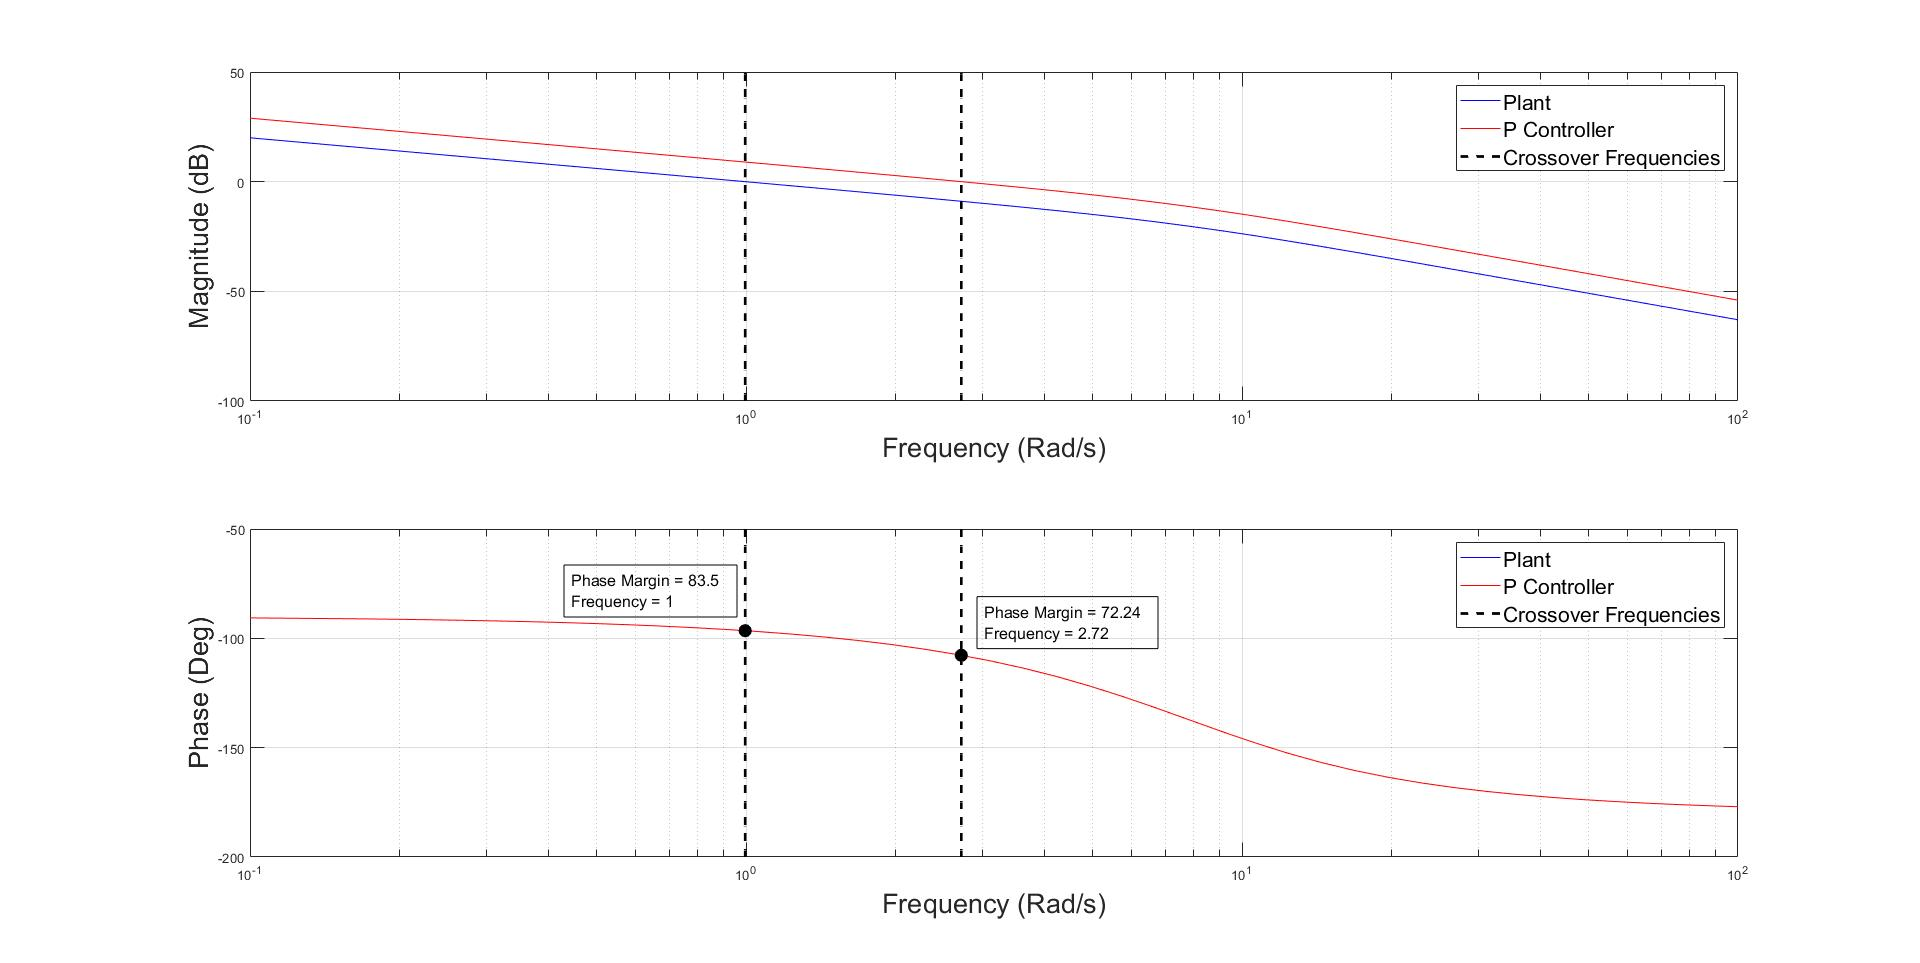
\includegraphics[height = 8cm]{../Design/Matlab/Controllers/climb_rate_bode.jpg}
		\caption{Climb Rate Controller - Open-Loop Bode Plots}
		\label{IM_ClimbRateBode}
	\end{figure}
	
	The bode plot shown in \ref{IM_ClimbRateBode} shows zero change in phase due to the controller architecture. The gain however is increased and moves the crossover frequency to $2.72 Rad/s$. The ratio of inner and outer loop crossover frequencies is then $2.91$, providing enough bandwidth between the inner and outer loops. The phase margin can then be calculated to be $72$\textdegree. 
	
	As shown in Figure \ref{IM_ClimbRateController} there is a limiter applied to the acceleration commands. This limit is present due to the confined operational environment and ensures that the climb rate controller does not saturate the horizontal velocity controllers. The final limits are shown in Table \ref{tab:ClimbrateLimits}
	
	\begin{table}[!]
		\centering
		\begin{tabular}{l | c | c |}
			Limit Name 						& Min & Max\\
			\hline\hline
			Acceleration Command 		    & -5 & 5 \\
		\end{tabular}
		\caption{Climb Rate Controller Limits}
		\label{tab:ClimbrateLimits}
	\end{table}
	
	\subsubsection{Climb Rate Controller Discussion}
	The dynamic response shows sufficient phase margin to handle unmodelled timing delays. While the ratio between the inner controller ensures this controller will not be attenuated. The step response of the closed loop system is shown in Figure \ref{IM_ClimbRateStep}. The system has a $5$\% settling time of $0.747s$ and shows negligible overshoot. At $5s$ a disturbance of $10N$ is placed on the rotors and the system demonstrates the ability to continue tracking the desired setpoint with zero steady state error.
	
	\begin{figure}[H]
		\centering
		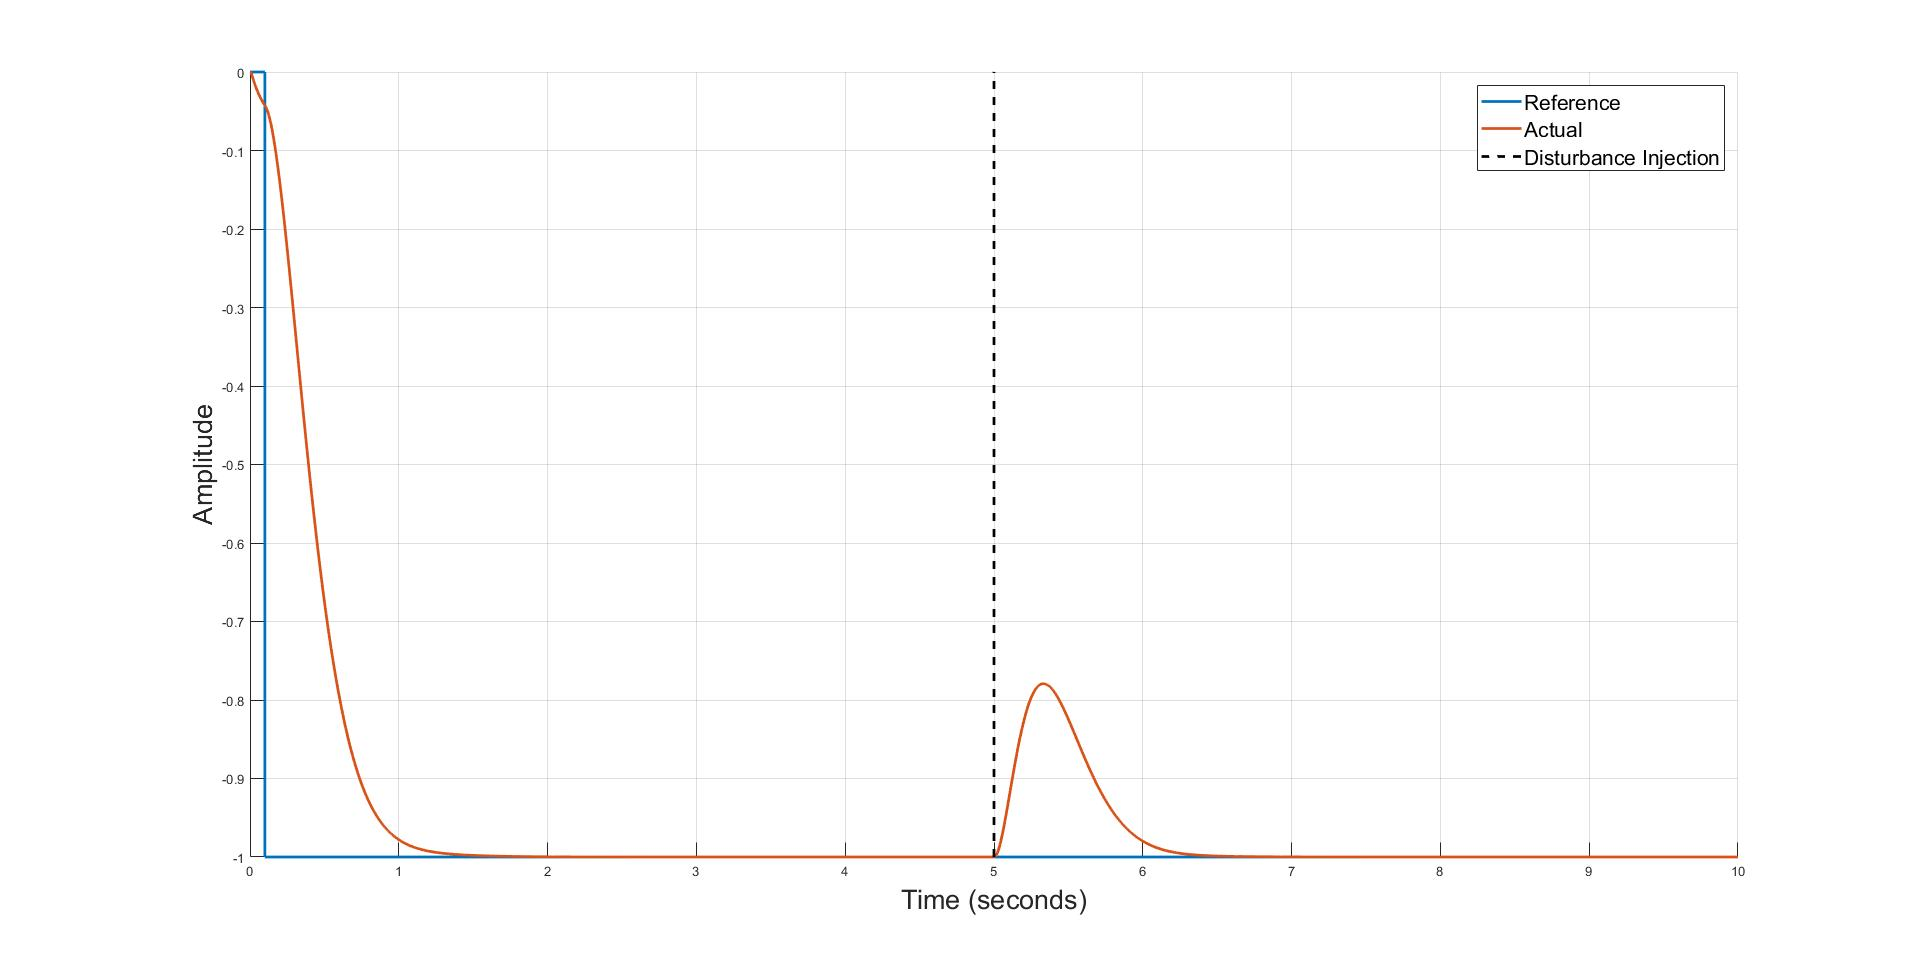
\includegraphics[height = 8cm]{../Design/Matlab/Controllers/climb_rate_step.jpg}
		\caption{Climb Rate Controller -  Step Response}
		\label{IM_ClimbRateStep}
	\end{figure}
	
	\subsection{Altitude Hold Controller}
	The final stage of the vertical control system is the altitude hold controller. This controller receives a desired altitude in the earth frame and outputs a reference velocity, also in the earth frame. The closed control loop block diagram is shown in Figure \ref{IM_AltHoldControlLoop}. This controller is limited by the response time of the inner loops and must be considered in the design.
	
	\begin{figure}[H]
		\centering
		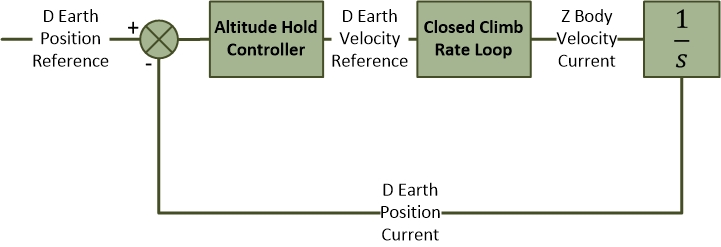
\includegraphics[height = 4cm]{../References/Diagrams/AltHoldLoop.jpg}
		\caption{Altitude Hold Controller Closed Loop}
		\label{IM_AltHoldControlLoop}
	\end{figure}
	
	The chosen controller architecture is shown in Figure \ref{IM_AltHoldController}. The proportional gain is used to vary the bandwidth to be within the limits of the system. The faded integrator shown in Figure \ref{IM_AltHoldController} is not considered during linear analysis. The integrator shall be limited in such a way as to limit the interference of the proportional gain. The reason for including the integrator is to ensure the system can track measurement errors in velocity with zero steady state error and exhibit a first order response. A PID controller architecture was also considered and the analysis was done for both control laws.
	
	The system's dynamic response is analysed using the root locus shown in Figure \ref{IM_AltHoldRoot} and the bode plot shown in Figure \ref{IM_AltHoldBode}.
	
	\begin{figure}[H]
		\centering
		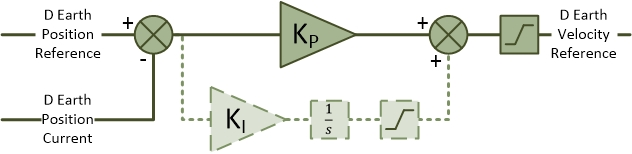
\includegraphics[height = 3.5cm]{../References/Diagrams/AltHoldController.jpg}
		\caption{Altitude Hold Controller}
		\label{IM_AltHoldController}
	\end{figure}
	
	Figures \ref{IM_AltHoldRoot} and \ref{IM_AltHoldBode} evaluate a P controller against a PID controller. The P controller adds no new poles or zeros and the closed loop poles of the P controlled system are placed at $-5.52 \pm 3.23i$ and $-2.03 \pm 0.58i$. 
	The PID controller adds an additional pole and two additional zeros into the system. The closed loop poles of the PID controlled system are located at $-6.64$, $-3.59 \pm 5.03i$ and $-0.64 \pm 0.47i$. The two new zeros are placed at $-0.57$ and $-2.06$.
	
	\begin{figure}[H]
		\centering
		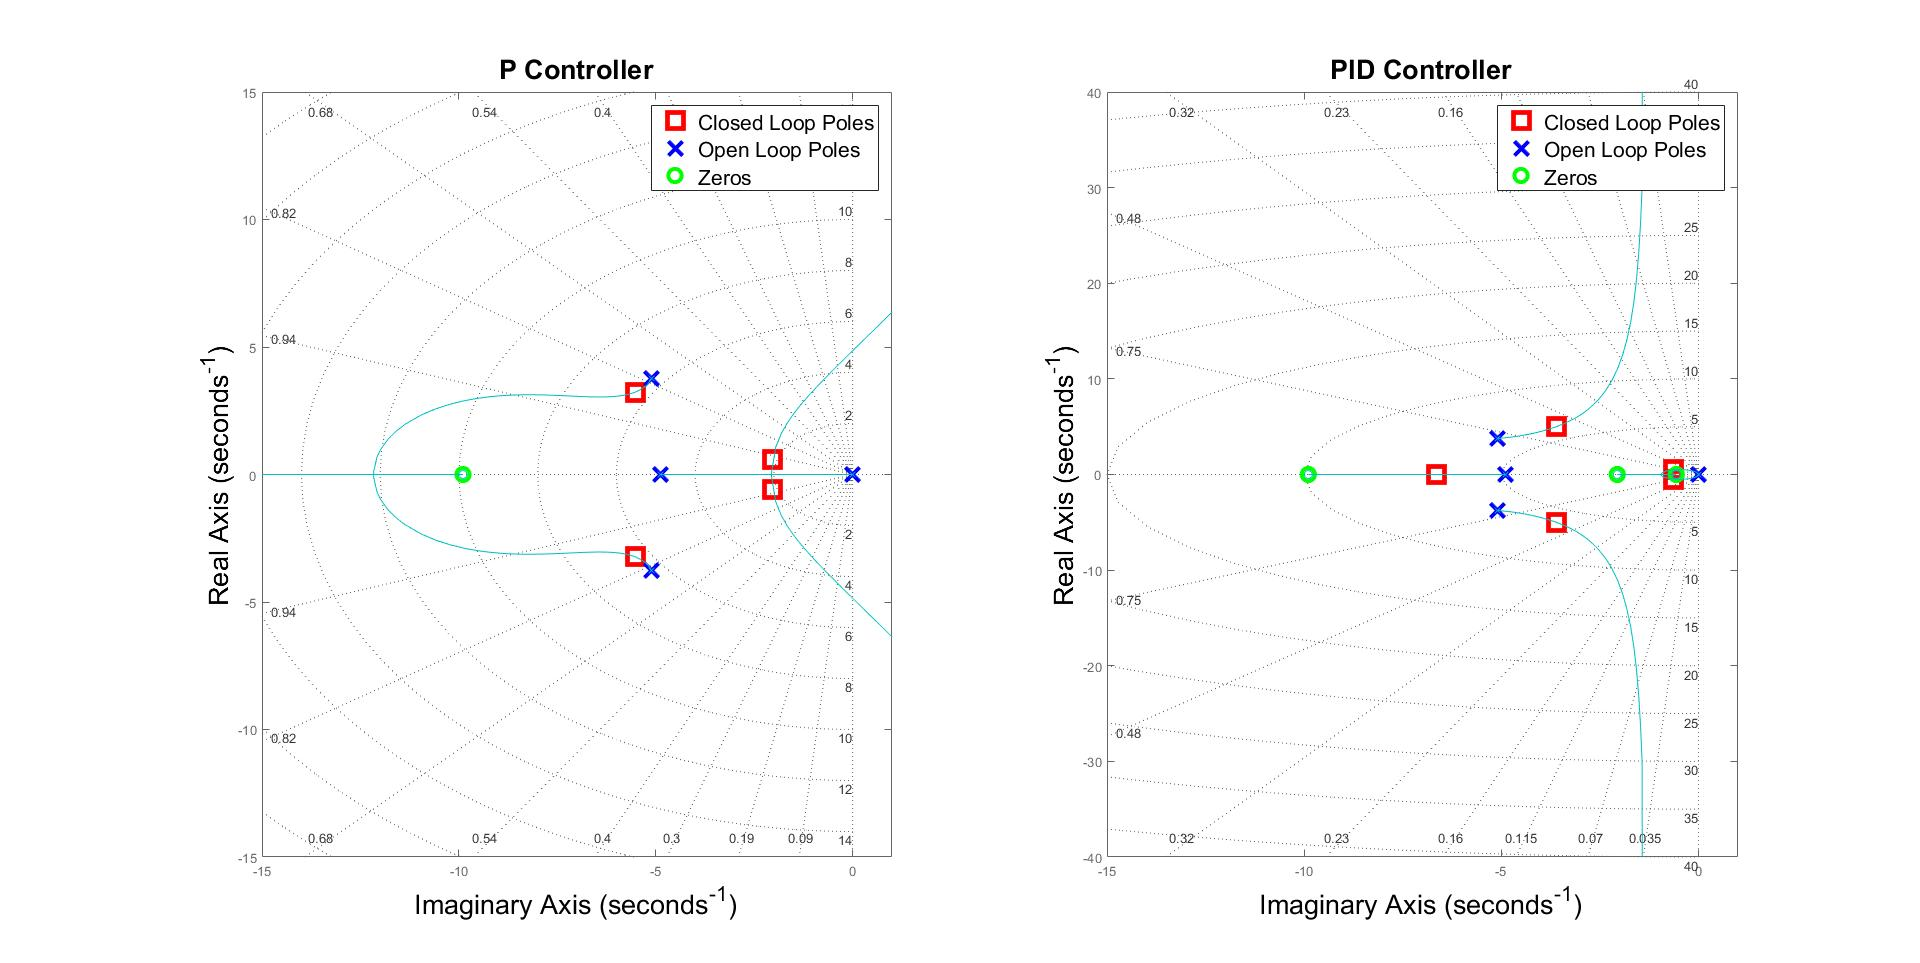
\includegraphics[height = 8cm]{../Design/Matlab/Controllers/altitude_root.jpg}
		\caption{Altitude Hold Controller -  Root Locus}
		\label{IM_AltHoldRoot}
	\end{figure}
	
	The bode plot shows the PID controller producing a final cross over frequency of $1.90Rad/s$, this response is too fast for the inner climb rate system and will need to be redesigned or discarded. The P controller exhibits a cross over frequency of $0.91Rad/s$, this produces a ratio of $3.03$ between the inner and outer loops and a phase margin of $71.5$\textdegree. The phase of the system using a P controller crosses the $180$\textdegree  $\ $mark at $4.81Rad/s$ and has a gain margin of $18.7dB$.
	
	\begin{figure}[H]
		\centering
		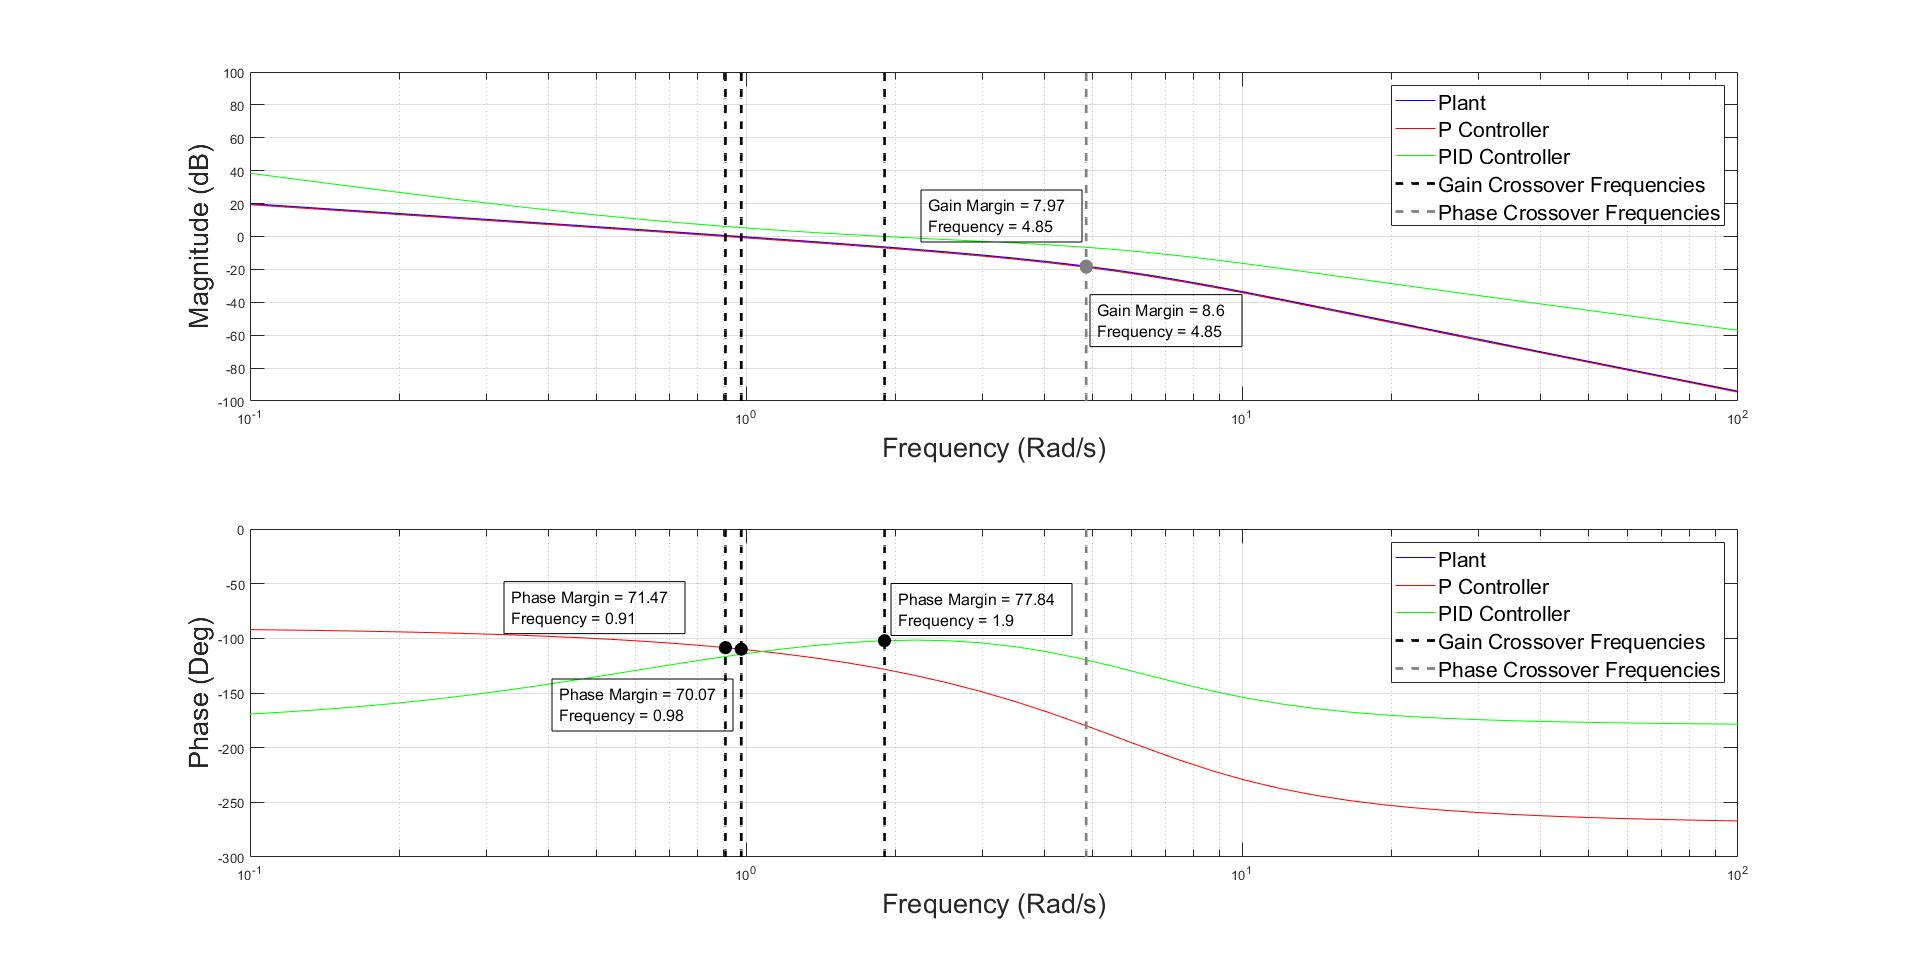
\includegraphics[height = 8cm]{../Design/Matlab/Controllers/altitude_bode.jpg}
		\caption{Altitude Hold Controller -  Bode Plots}
		\label{IM_AltHoldBode}
	\end{figure}
	
	To finalise the design, the two limiters are discussed. The first limiter is used to limit the effect of the integrator on the system as well as stop integrator wind up. The second limiter is used to limit the climb rate commands sent to the inner controllers. Both sets of limits are shown in Table \ref{tab:AltitudeControllerLimits}
	
	\begin{table}[!]
		\centering
		\begin{tabular}{l | c | c |}
			Limit Name 						& Min & Max\\
			\hline\hline
			Integrator Wind Up 				& -0.09 & 0.09 \\
			Climb Rate Command 		    	& -5 & 5 \\
		\end{tabular}
		\caption{Altitude Hold Controller Limits}
		\label{tab:AltitudeControllerLimits}
	\end{table}
	
	\subsubsection{Altitude Hold Controller Discussion}
	Although both the P and PID controllers exhibit stable dynamic responses, the PID controller exhibited too fast a response and will be effected by the inner controllers. The system including only a P controller exhibits a step response as shown in Figure \ref{IM_AltHoldStep}, a disturbance of $10N$ is applied to the rotors at $10s$. The system has a $5\%$ settling time of $2.29s$ and tracks the set point with zero steady state error. The system handles the disturbance with a maximum overshoot of $0.01m$ and is critically damped.
	
	\begin{figure}[H]
		\centering
		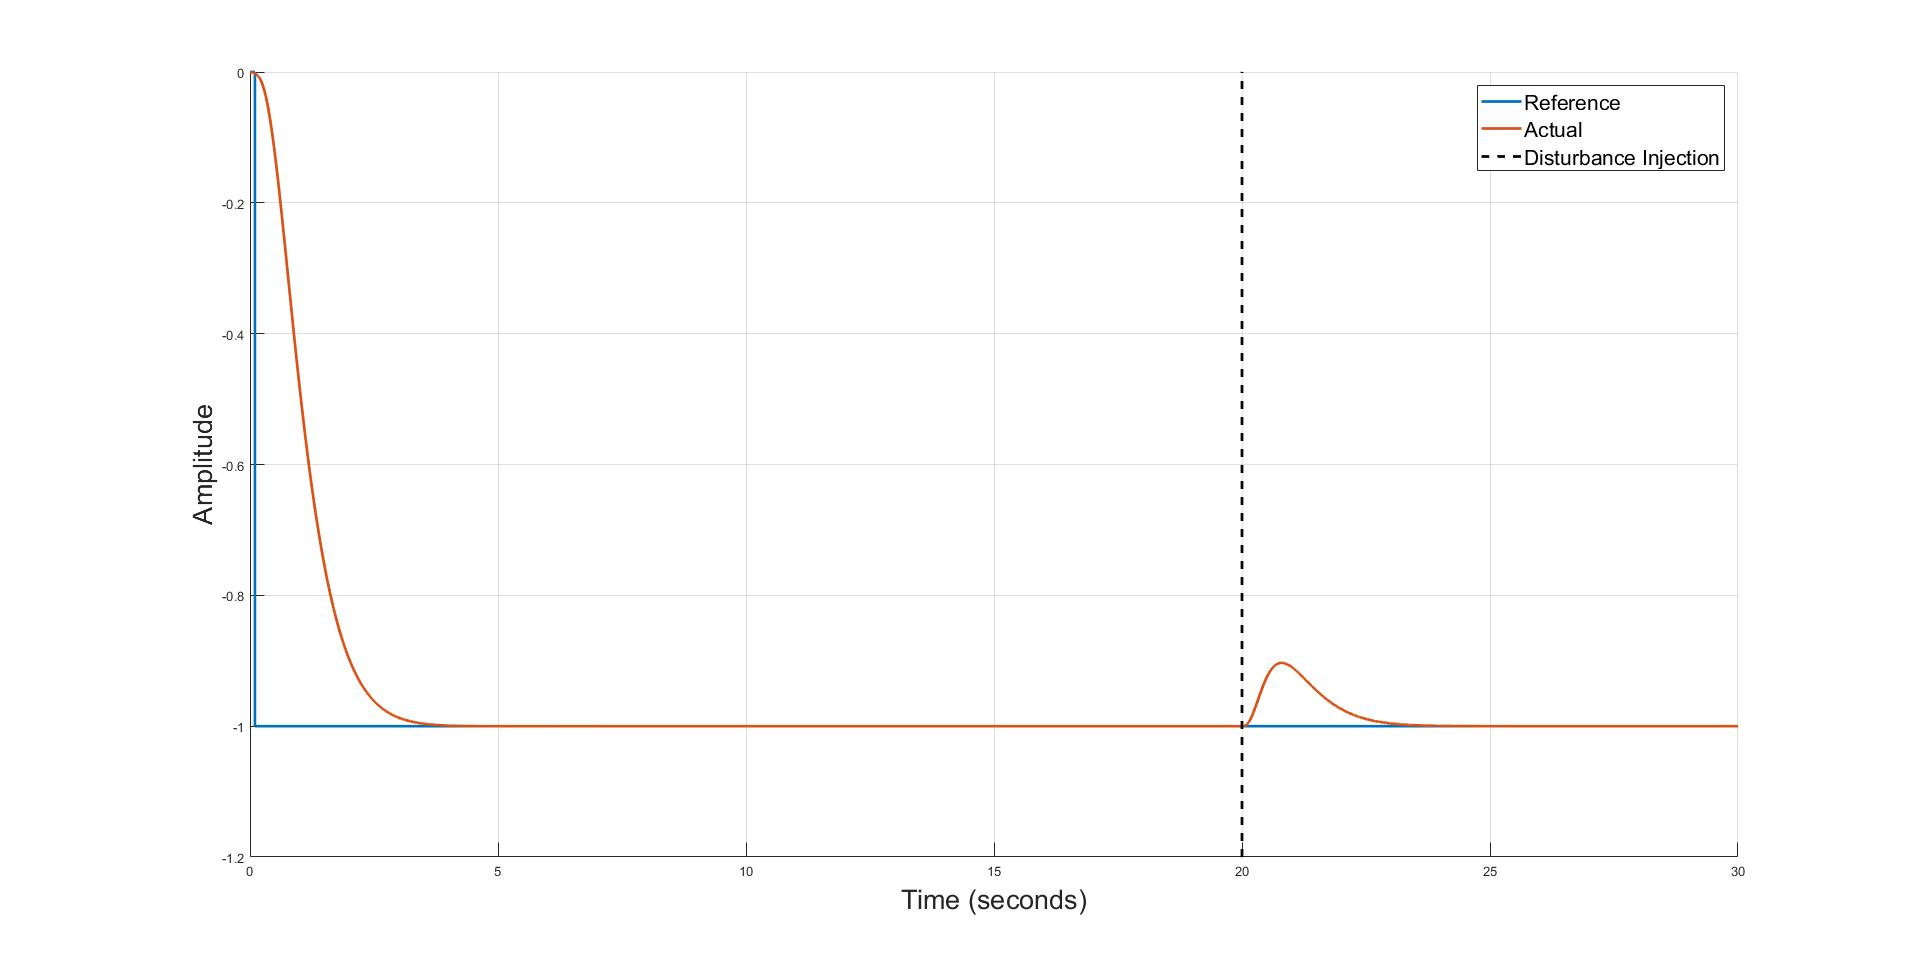
\includegraphics[height = 8cm]{../Design/Matlab/Controllers/altitude_step_p_no_dist.jpg}
		\caption{Altitude Hold P Controller -  Step response}
		\label{IM_AltHoldStep}
	\end{figure}
	
	However, if a measurement disturbance is present in the inner loops, this system will not track a setpoint with zero steady state error. To demonstrate this a constant offset of $0.05m/s$ is placed on the Z-Axis velocity measurement, Figure \ref{IM_AltHoldPDistStep} shows the current system cannot account for this disturbance. As shown in \ref{IM_AltHoldController}, a limited gain integrator is introduced into the system to help the system track steady state error. 
	
	\begin{figure}[H]
		\centering
		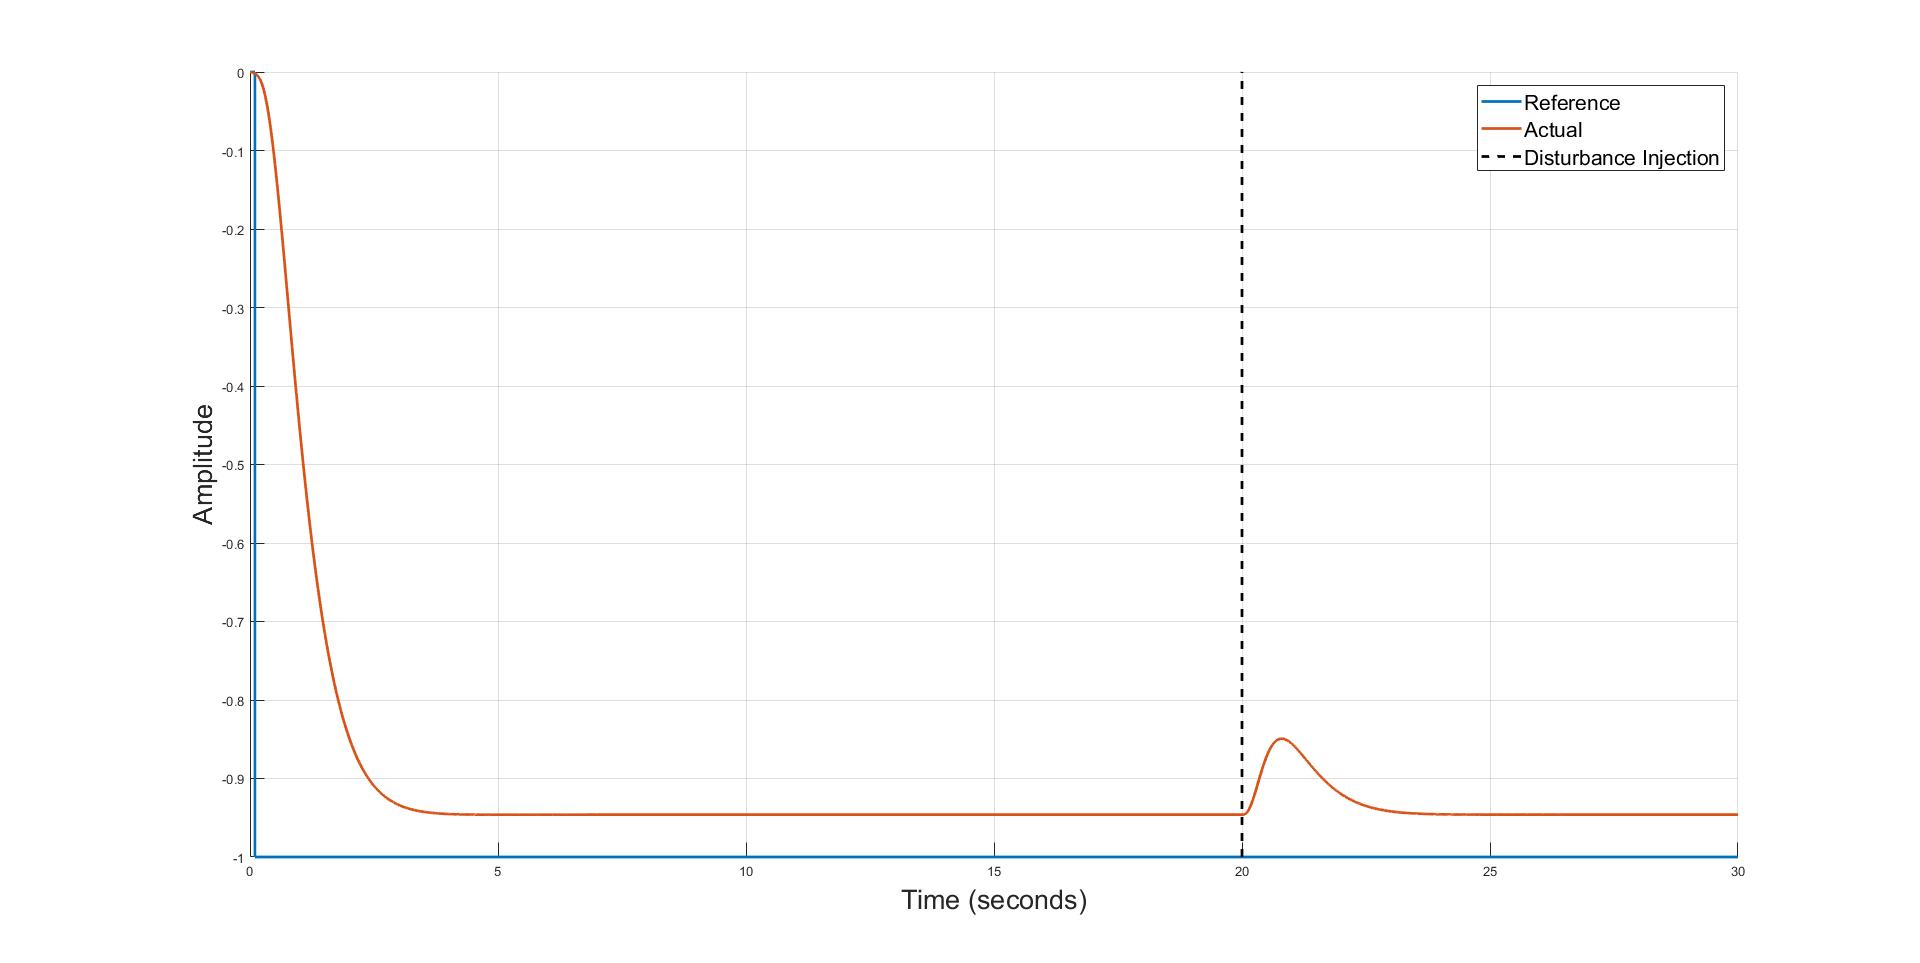
\includegraphics[height = 8cm]{../Design/Matlab/Controllers/altitude_step_p_dist.jpg}
		\caption{Altitude Hold P Controller -  Step response with inner loop measurement offset}
		\label{IM_AltHoldPDistStep}
	\end{figure}
	
	The new controller must be limited in such a way as to exhibit a similar transient response as the existing P controller. Figure \ref{IM_AltHoldPIDistStep} shows the step response of the new system both with and without the $0.05m/s$ offset in the velocity measurement. As shown, the P controller including a limited I component introduces more overshoot into the system. The limits are designed to ensure the new controller introduces less than 10\% overshoot into the system. 
	
	\begin{figure}[H]
		\centering
		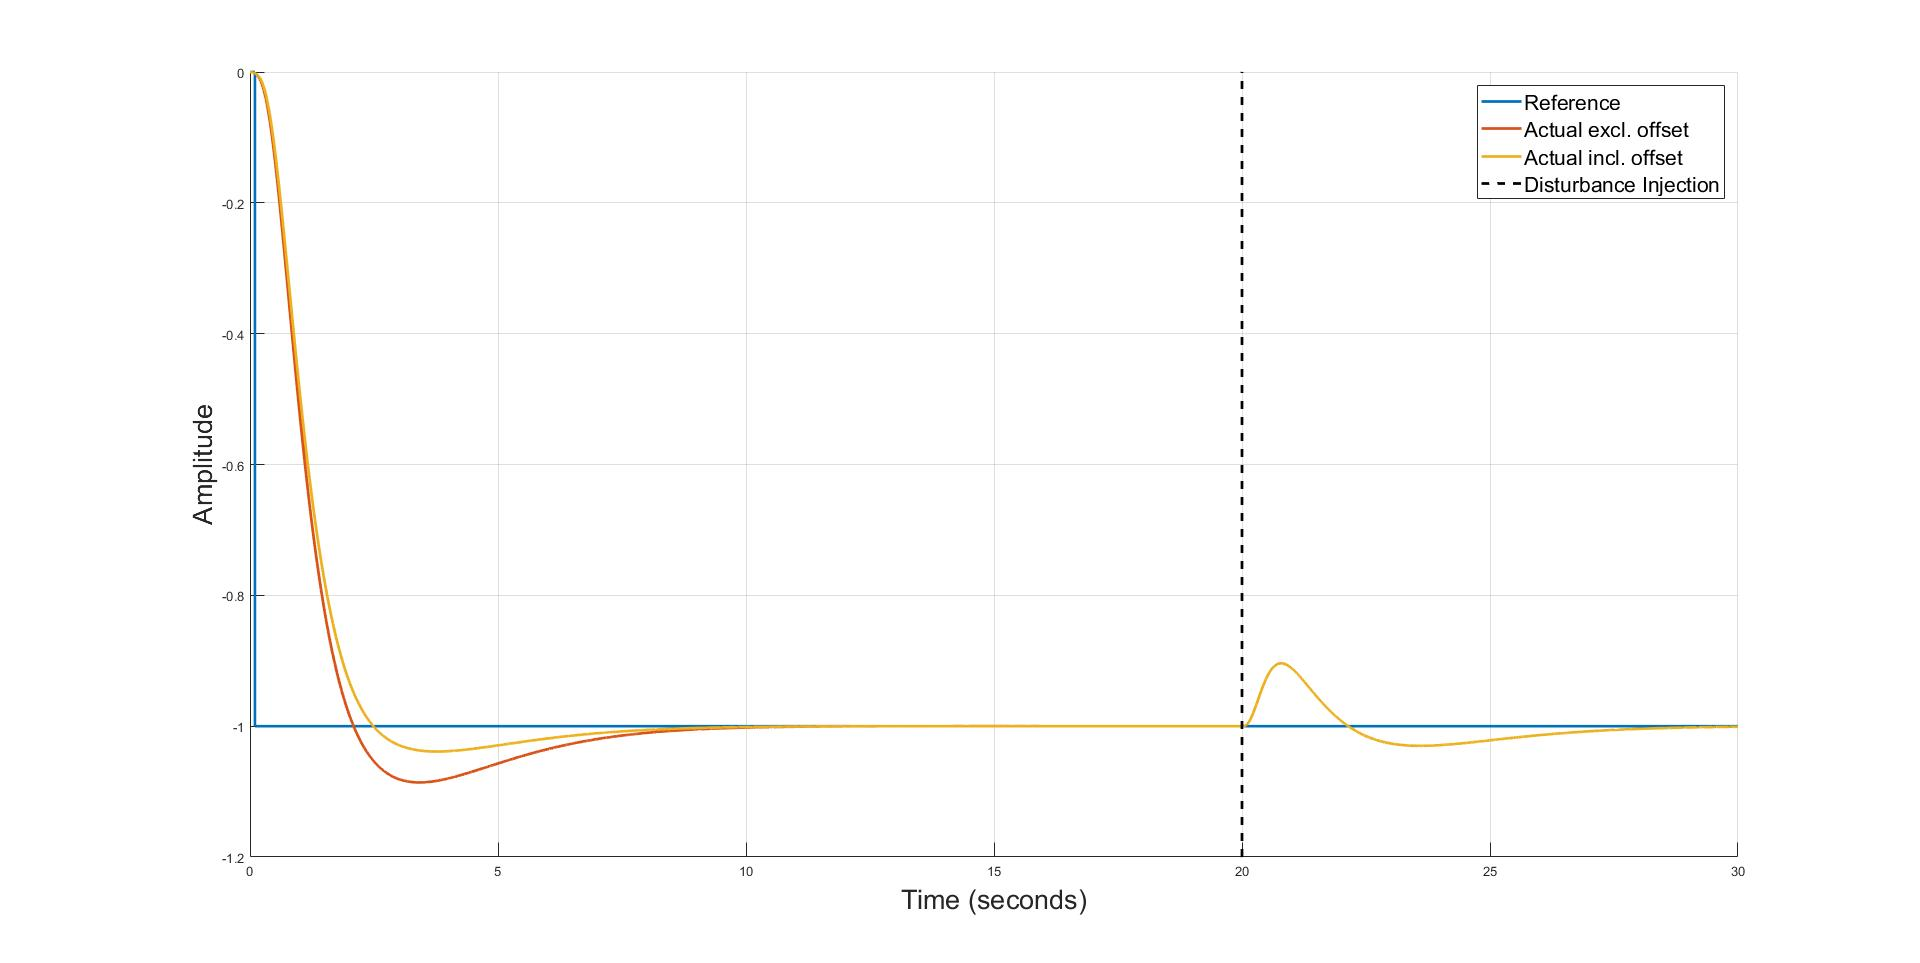
\includegraphics[height = 8cm]{../Design/Matlab/Controllers/altitude_step_pi.jpg}
		\caption{Altitude Hold P with Limited I Controller -  Step Responses}
		\label{IM_AltHoldPIDistStep}
	\end{figure}

		
	\end{document}   